\subsection{Plain circuit}
\label{sec:plain}

Creating the LTSpice model of the plain circuit set the baseline for all further work. Interpreting Figure \ref{fig:schematic_altium_1} and \ref{fig:schematic_altium_2} yielded what can be seen in Figure \ref{fig:spice_plain_1}. The original converter has about $900V$ over the power pole, so a symmetric 450V supply was chosen.

\begin{figure}[H]
	\centering
	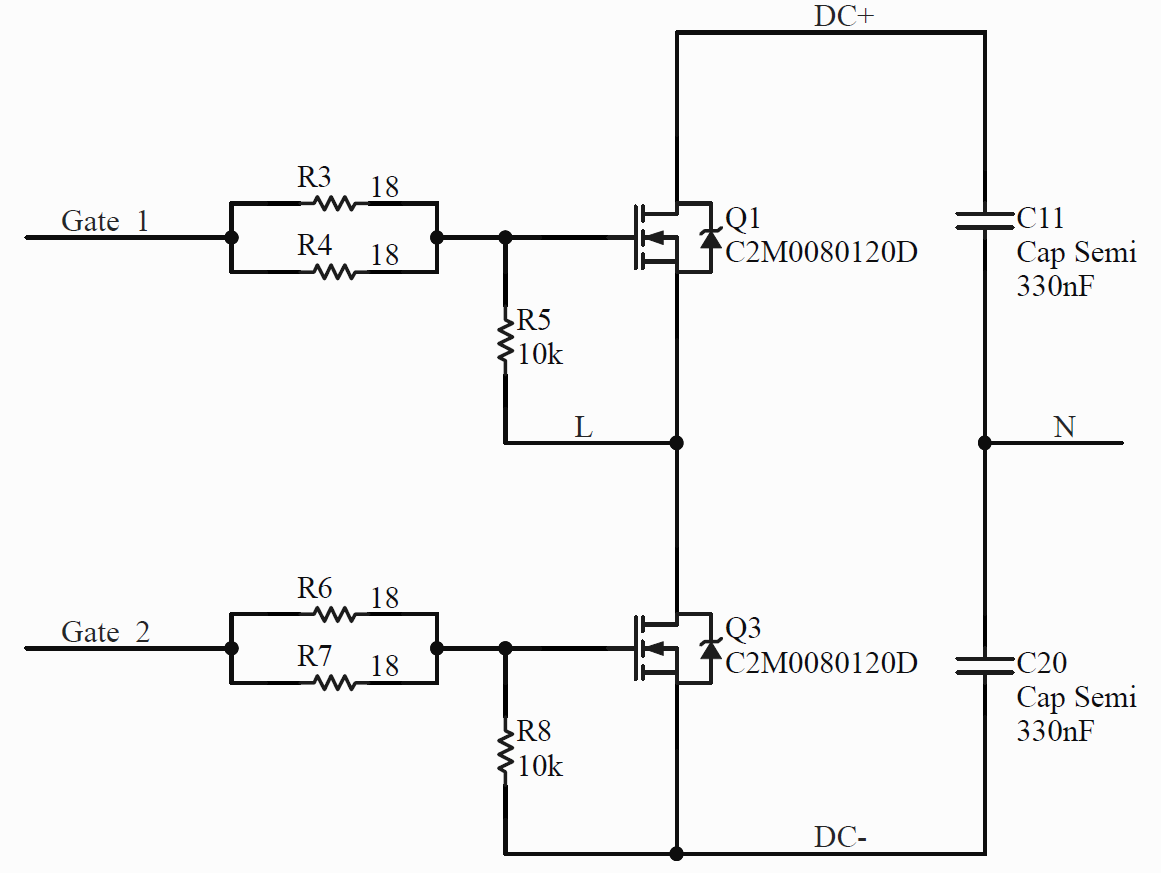
\includegraphics[width=\textwidth]{pictures/implementation/schematic_altium_1.PNG}
	\caption{Schematic of power pole}
	\label{fig:schematic_altium_1}
\end{figure}

\begin{figure}[H]
	\centering
	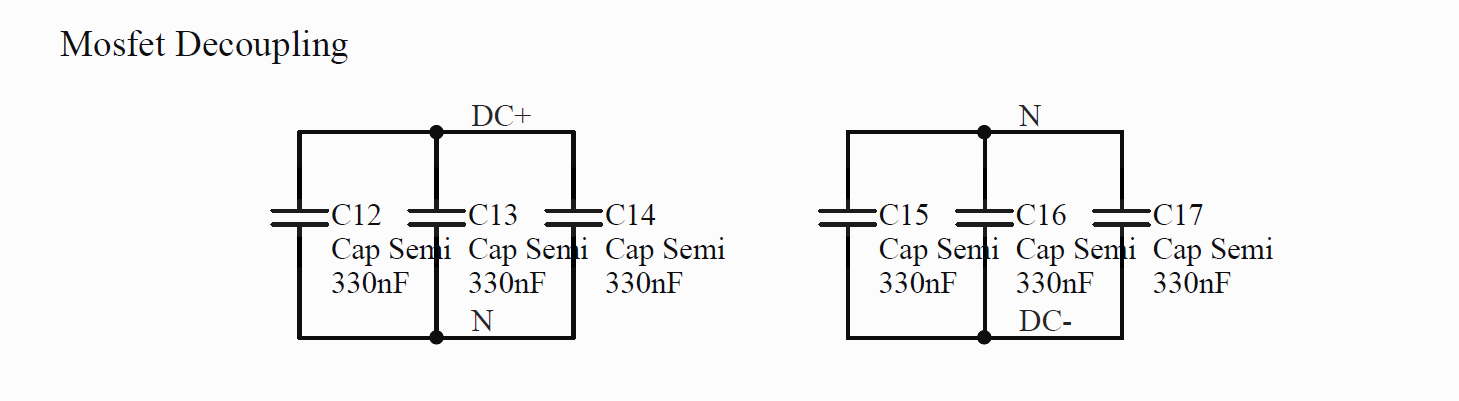
\includegraphics[width=\textwidth]{pictures/implementation/schematic_altium_2.PNG}
	\caption{Decoupling capacitors parallel to C11 and C20}
	\label{fig:schematic_altium_2}
\end{figure}

\begin{figure}[H]
	\centering
	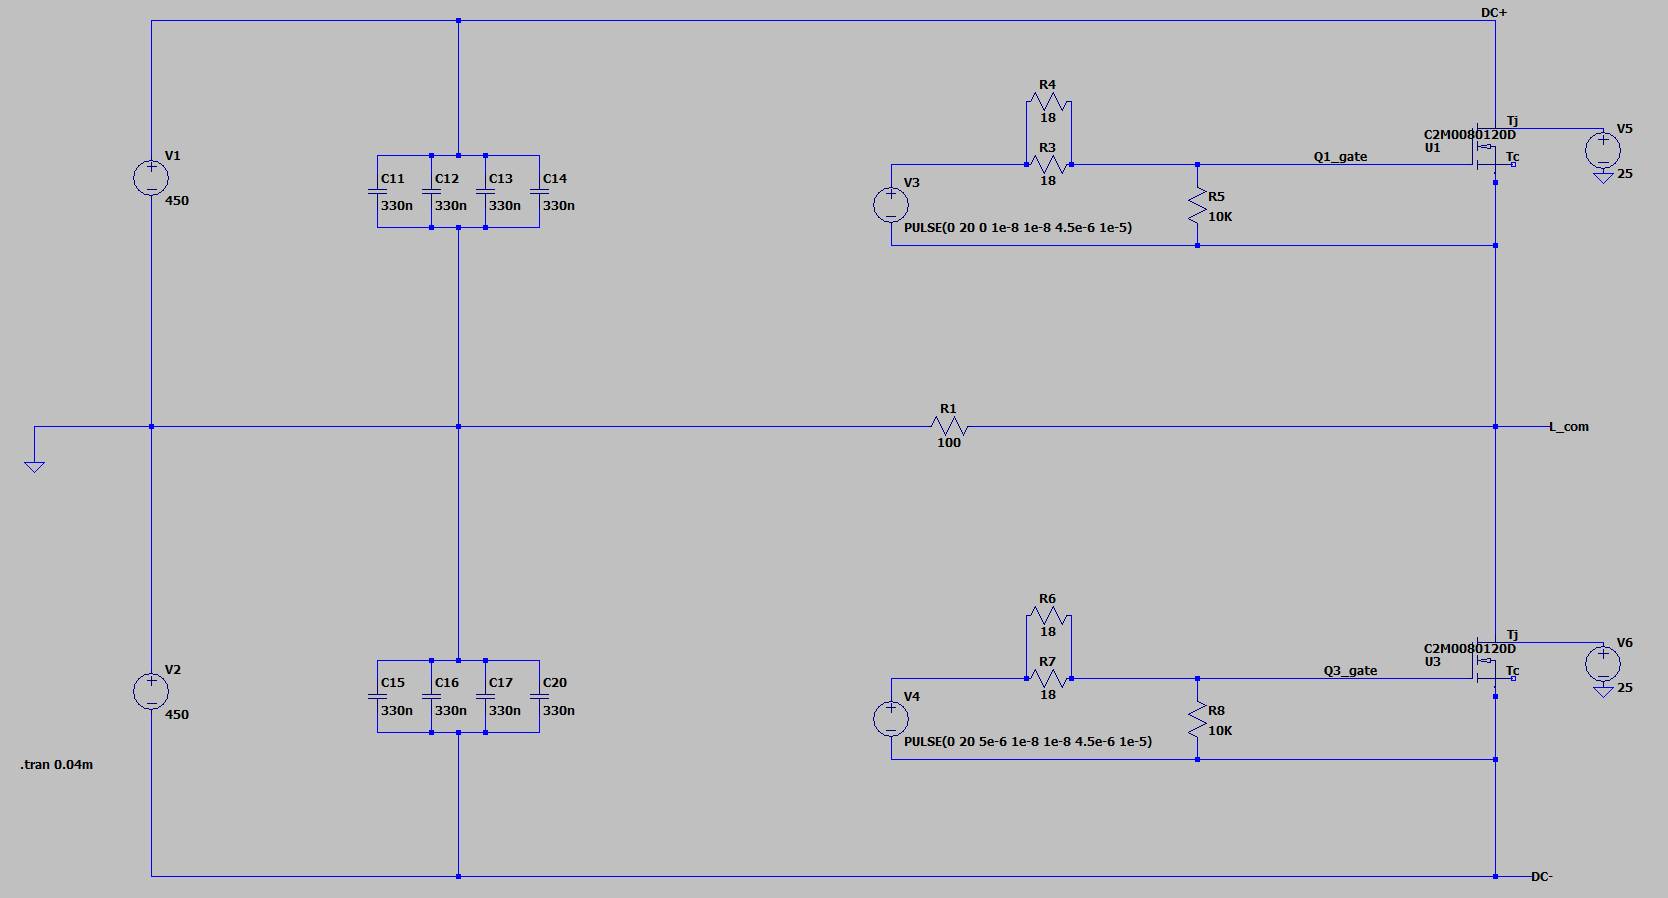
\includegraphics[width=\textwidth]{pictures/implementation/plain/spice_plain_1.PNG}
	\caption{LTSpice model of plain circuit}
	\label{fig:spice_plain_1}
\end{figure}

The only nonideality in this circuit is the manufacturer model \cite{mosfet_2} of the MOSFET Cree C2M0080120D. As most of the gate-source voltage dependent parameters were specified at $V_{GS} = 20V$ in its datasheet \cite{mosfet}, a $V_{GS} = 20V$ was chosen. The original converter runs at a switching frequency of $100 kHz$, so it was natural to pick that. On and off slopes should be quick enough to challenge the layout, so they were chosen to be 2 orders of magnitude quicker than the period time. 10\% deadtime was also included to prevent shoot-through at switching.\\

The MOSFET model supports thermal simulation that has not been utilized. The junction temperature $T_j$ was fixed at 25\textcelsius.

\subsubsection{Waveforms}
\label{sec:plain_waveforms}

The simulated waveforms look plausible. Some cross-coupling can be seen at the moment of the switching but this is not enough to trigger false turn on-off cycles.

Figure \ref{fig:plain_gates_1} shows two whole cycles as an overview, Figure \ref{fig:plain_gates_2} shows the transient where $ Q_1$ $V_{GS}$ turns off, Figure \ref{fig:plain_gates_3} depicts the other end of that cycle. Figure \ref{fig:plain_load} demonstrates the voltage and current of the load.

\begin{figure}[H]
	\centering
	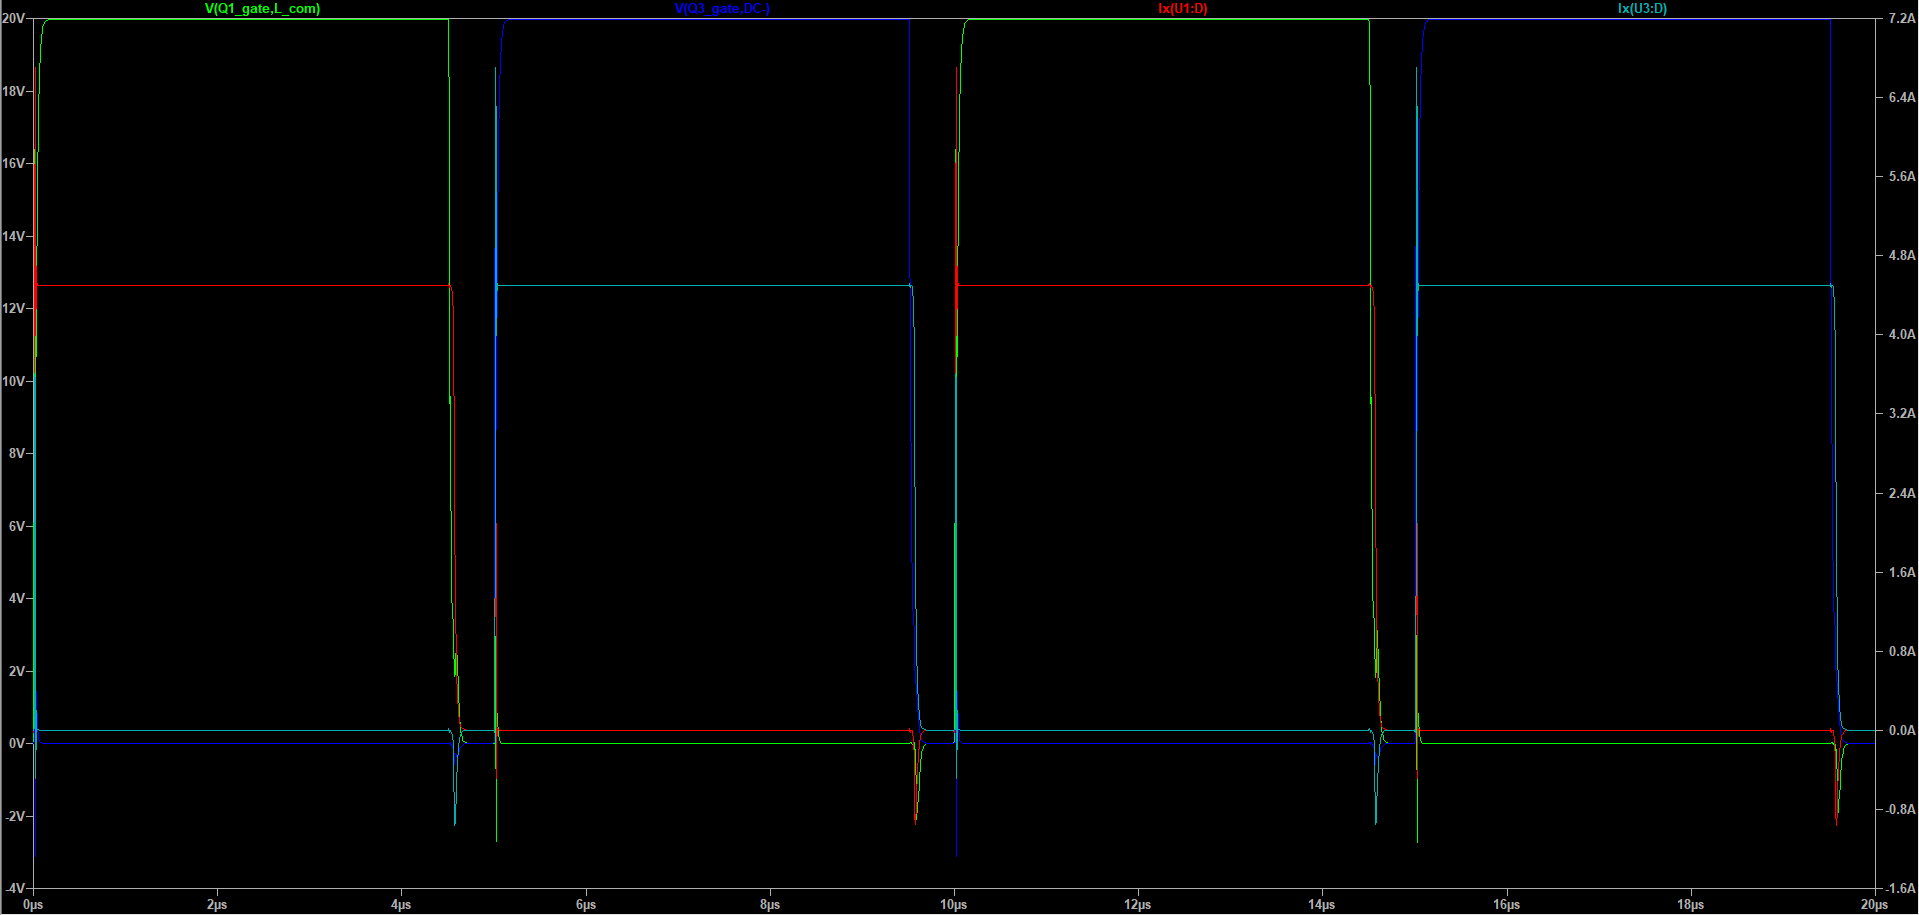
\includegraphics[width=\textwidth]{pictures/implementation/plain/plain_gates_1.PNG}
	\caption{Overview of the gate voltages and drain currents}
	\label{fig:plain_gates_1}
\end{figure}

\begin{figure}[H]
	\centering
	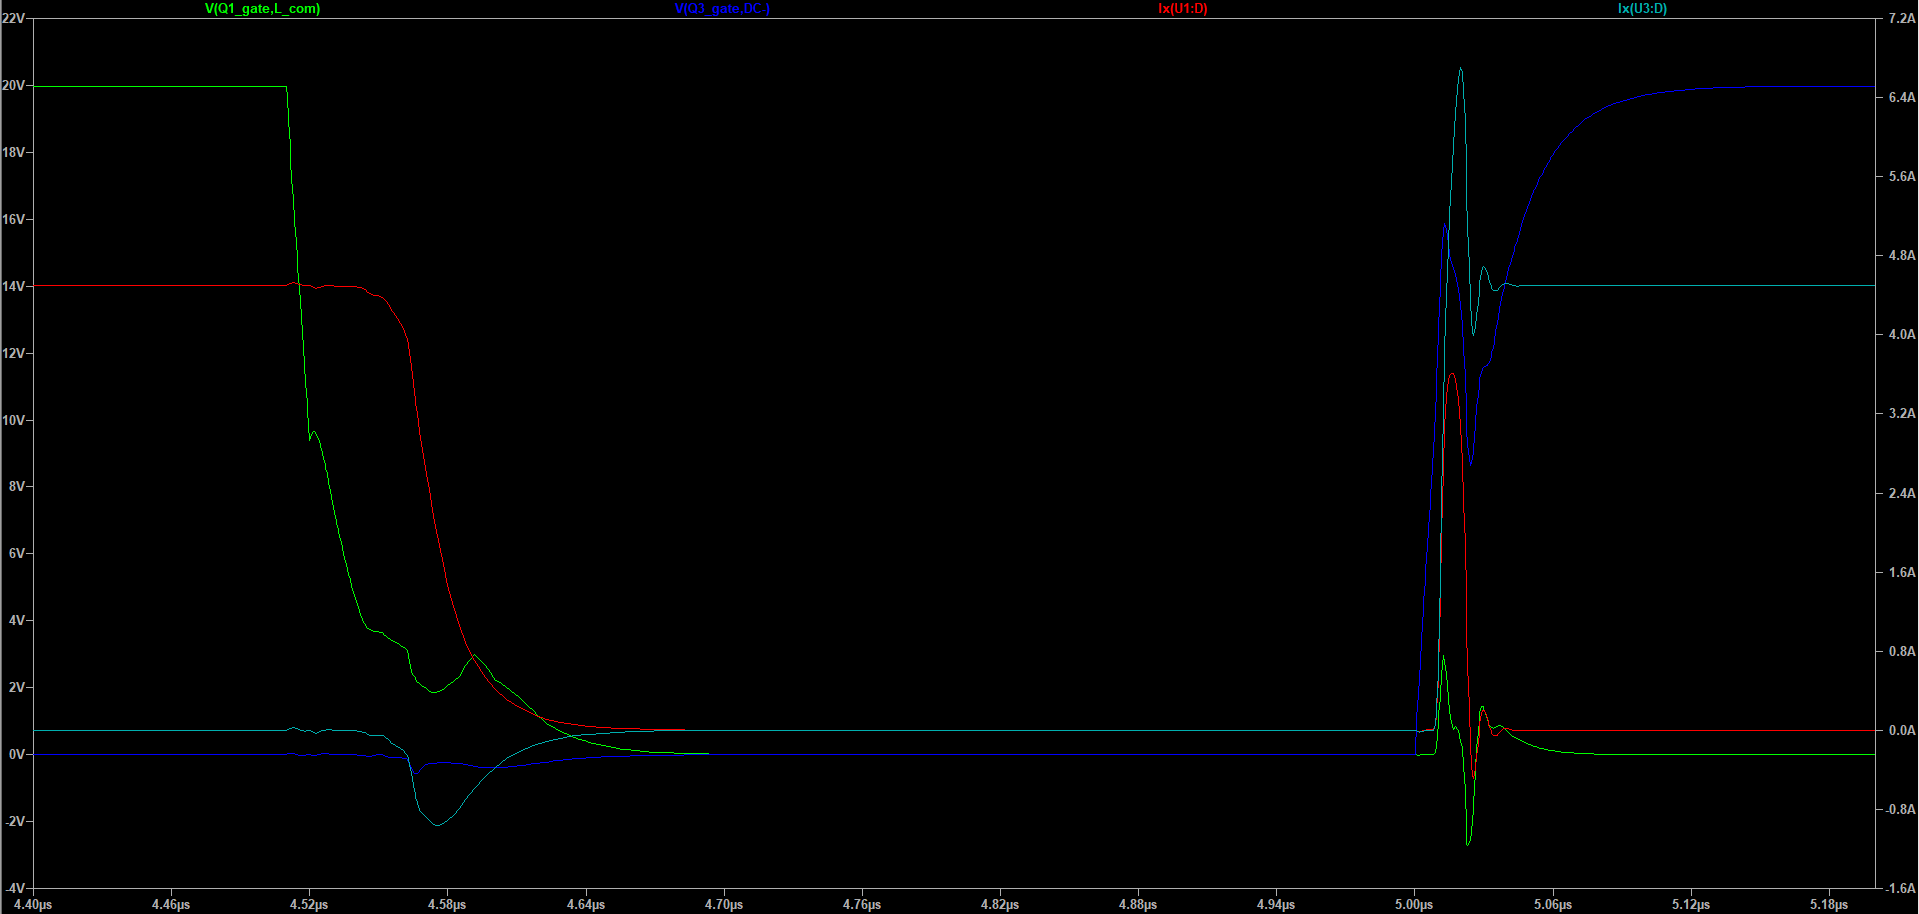
\includegraphics[width=\textwidth]{pictures/implementation/plain/plain_gates_2.PNG}
	\caption{Q1 turn off transient, gate voltages and drain currents}
	\label{fig:plain_gates_2}
\end{figure}

\begin{figure}[H]
	\centering
	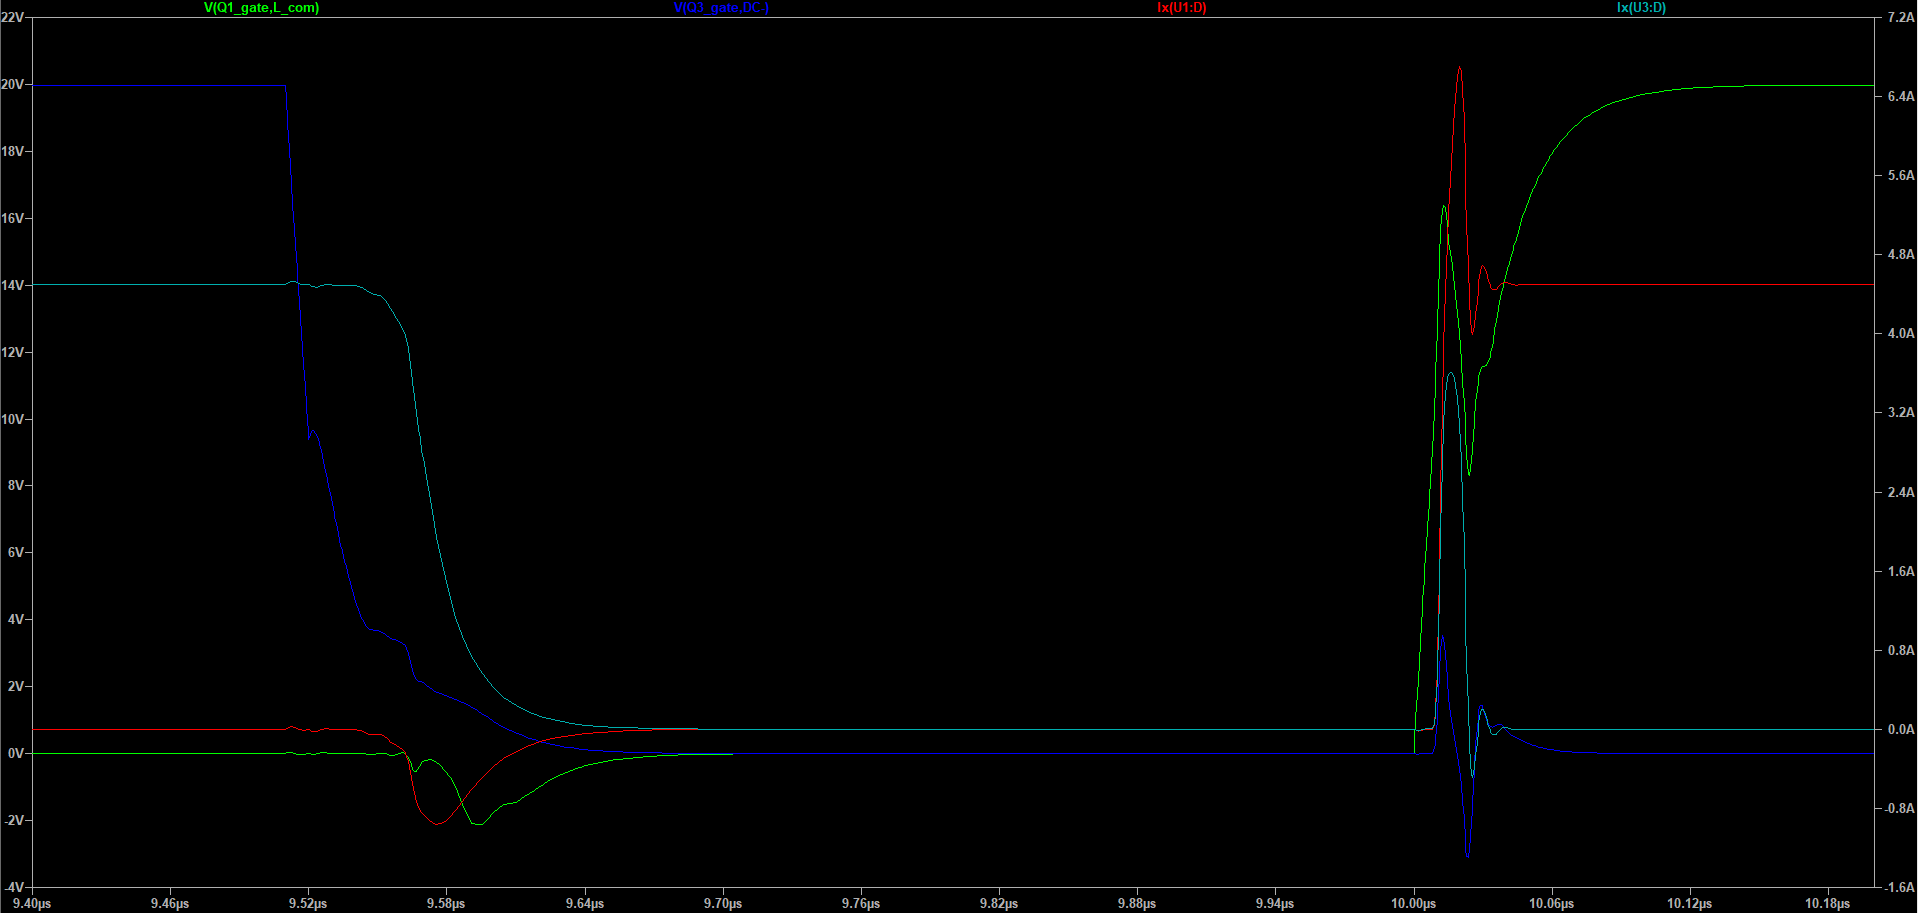
\includegraphics[width=\textwidth]{pictures/implementation/plain/plain_gates_3.PNG}
	\caption{Q3 turn off transient, gate voltages and drain currents}
	\label{fig:plain_gates_3}
\end{figure}

\begin{figure}[H]
	\centering
	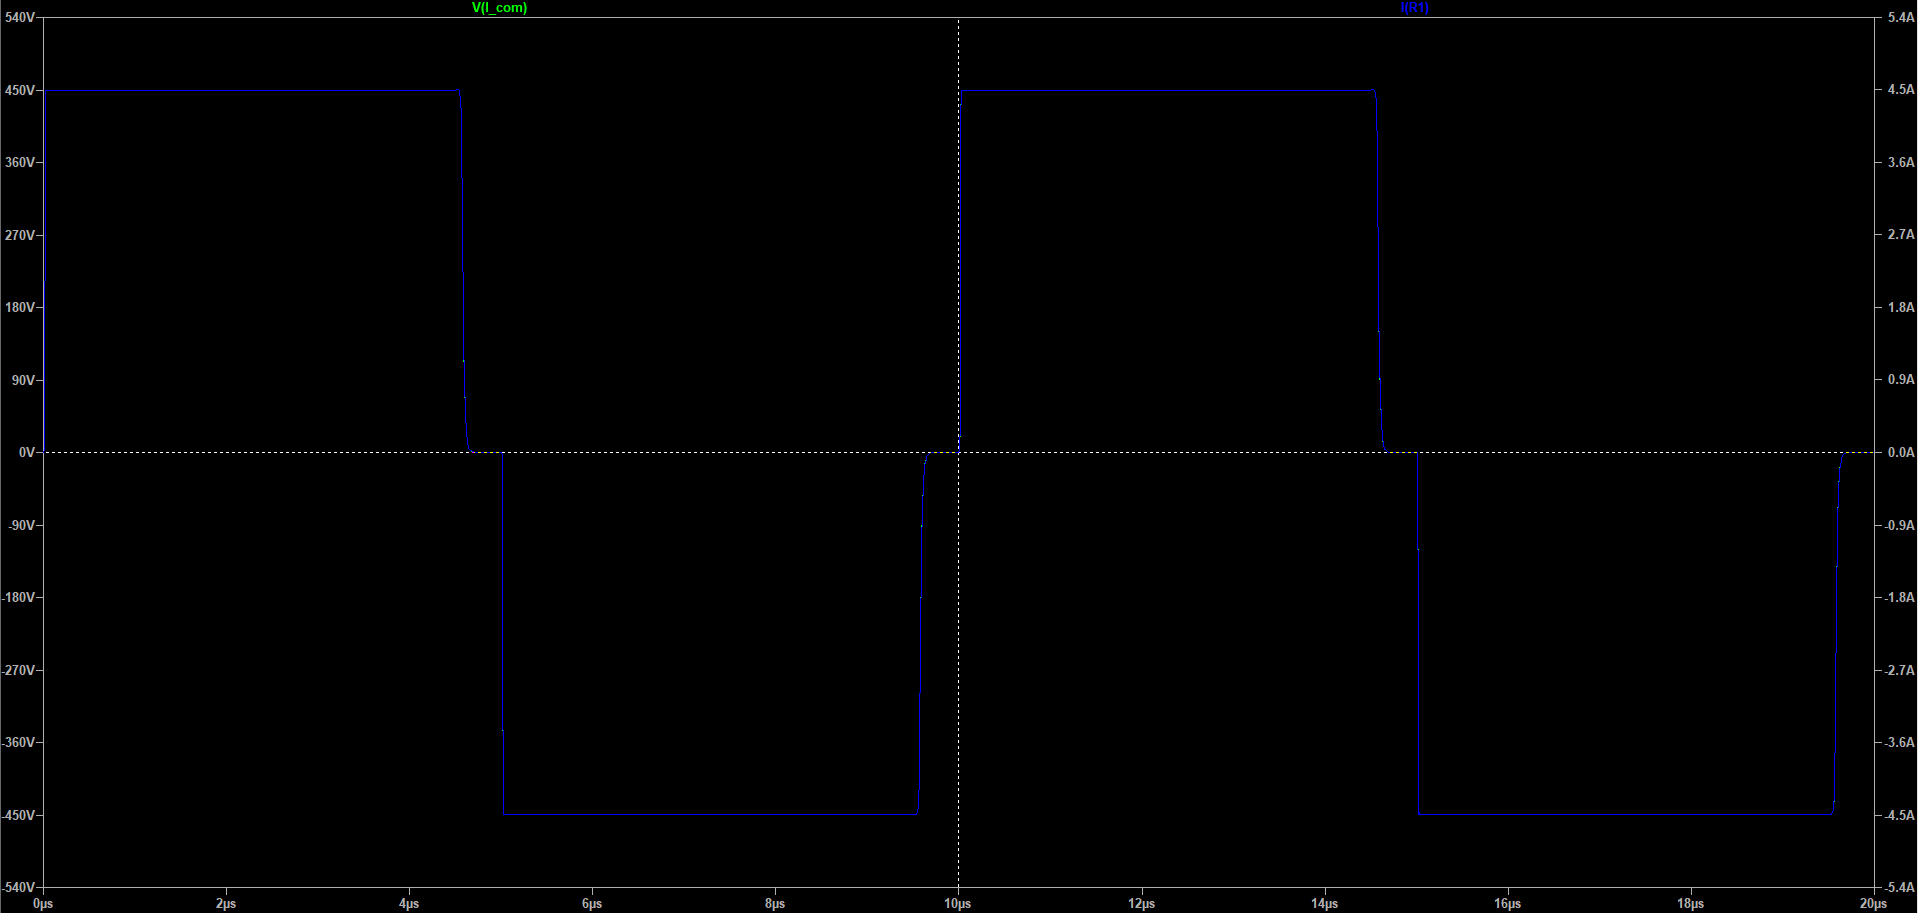
\includegraphics[width=\textwidth]{pictures/implementation/plain/plain_load.PNG}
	\caption{Voltage and current waveforms of the resistor overlap}
	\label{fig:plain_load}
\end{figure}